\documentclass[11pt,a4paper,oneside]{article}

\title{\textbf{RouteToDam: Provide information on day trips to Rotterdam for students at Utrecht University}\newline \newline \newline}
\date{\today}
\author{Sorin Dragan, Evangelia Giannikou, \\Mikhail Ternyuk, Olusanmi Hundogan}
\pagenumbering{gobble}
\usepackage{eurosym}
\usepackage{hyperref}
\usepackage{amsmath}
\usepackage{amssymb}
\usepackage{tabularx,booktabs}
\usepackage{multicol}
\usepackage{array}
\usepackage{float}
\usepackage[english]{babel}
\usepackage{quoting}
\usepackage{csquotes}
\usepackage{enumitem}
\usepackage{natbib}
\usepackage{xcolor}
\usepackage{subfiles}
\usepackage{ragged2e}
\usepackage{lmodern,textcomp}
\usepackage{graphicx}
\usepackage{titling}
\newcolumntype{M}[1]{>{\centering\arraybackslash}m{#1}}
\usepackage[backend=biber, sorting=none]{biblatex}
\usepackage[total={6.5in, 10in}]{geometry}
\addbibresource{references.bib}

\begin{document}

\maketitle


\begin{figure}[H]
    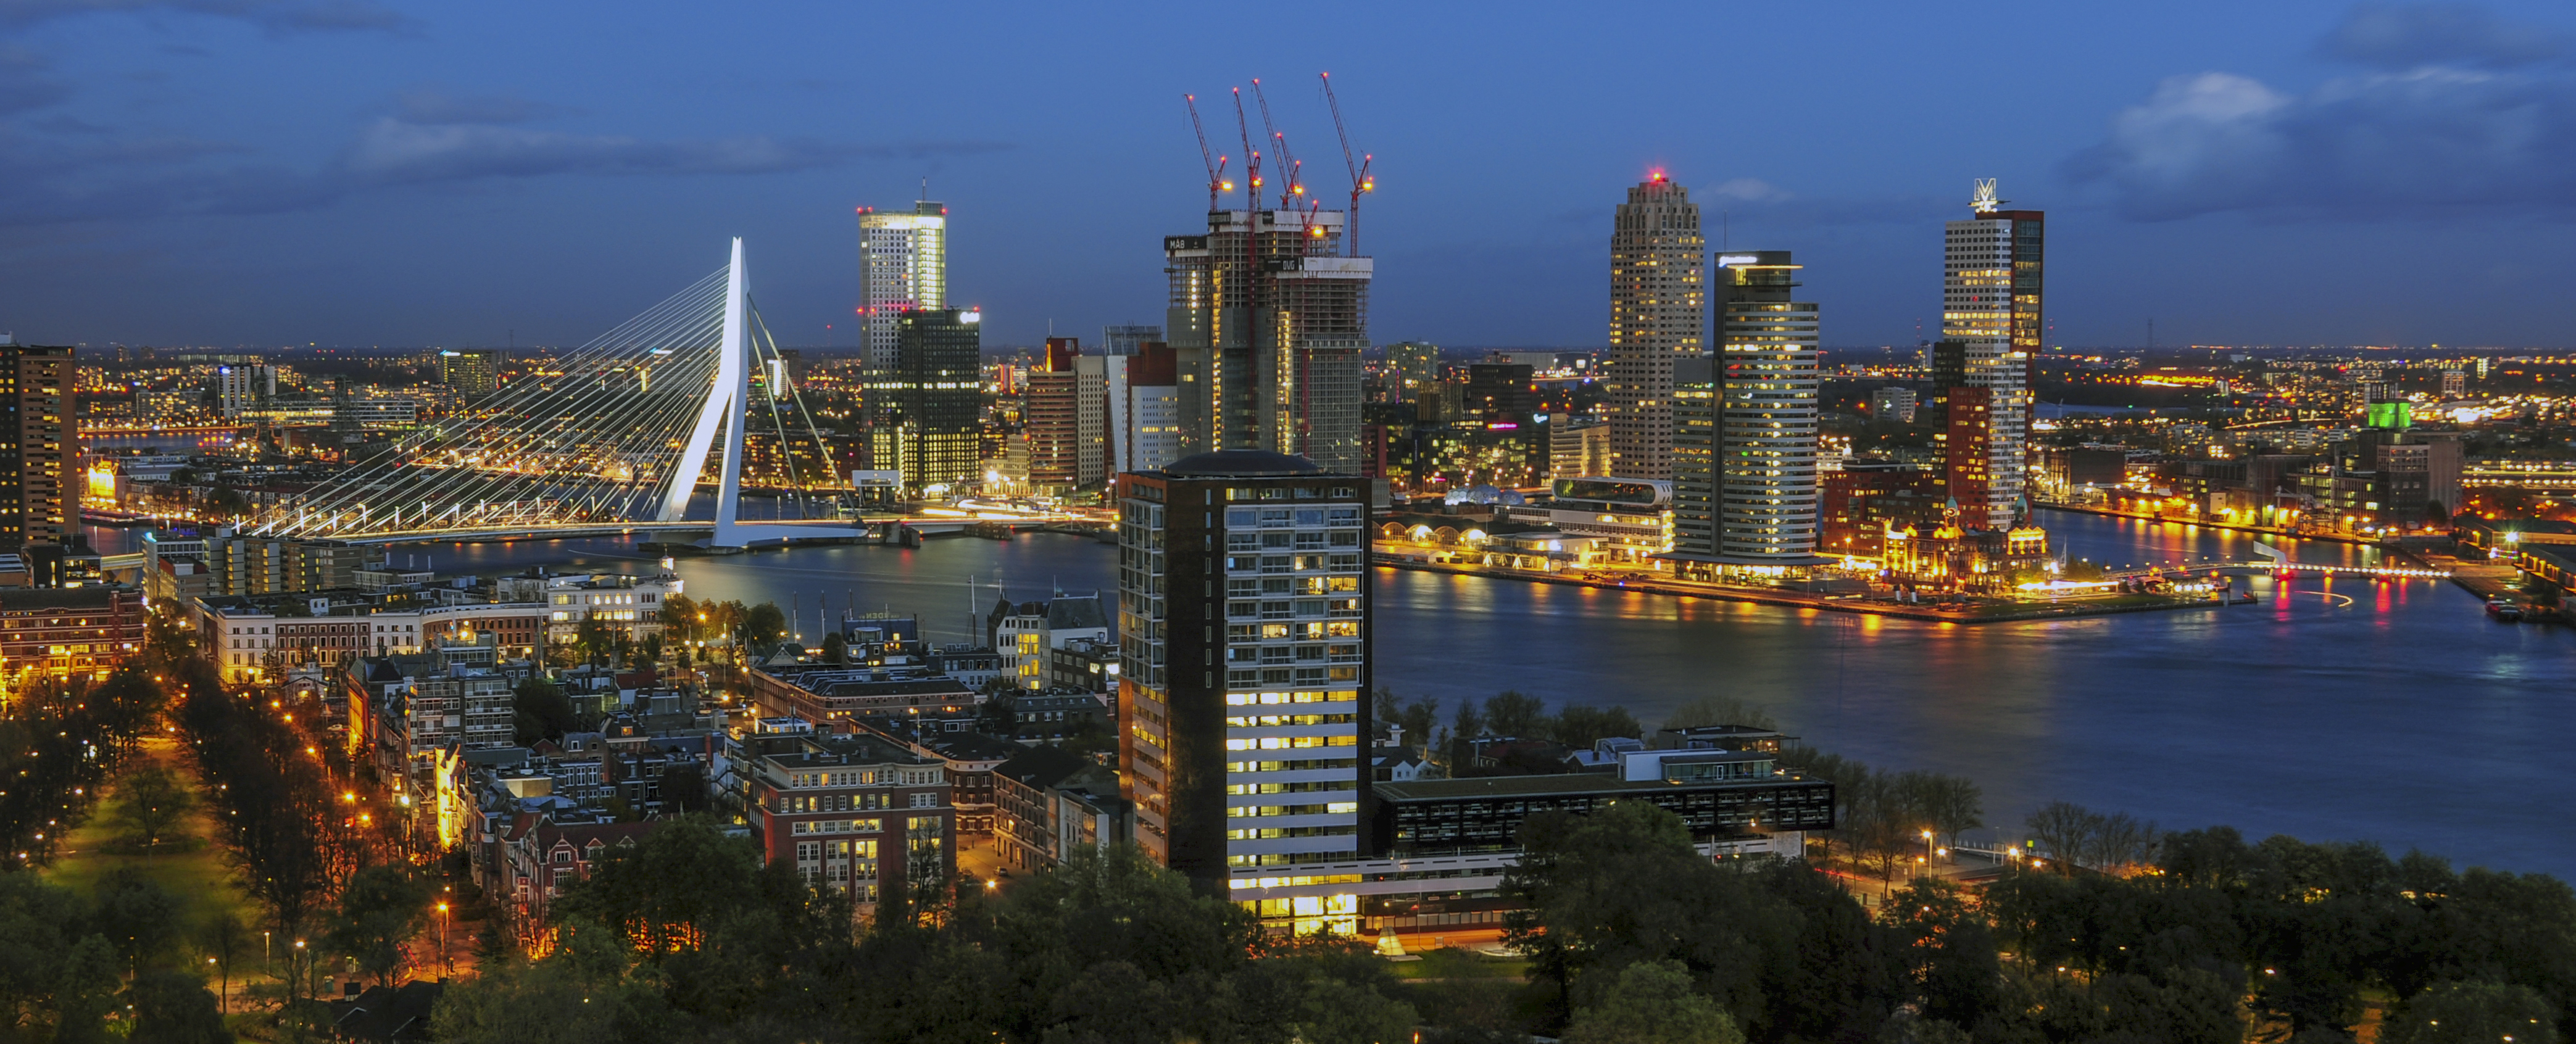
\includegraphics[width=\textwidth]{paper/imgs/Erasmusbrug_seen_from_Euromast.jpg}
    \caption{An upfront view of Rotterdam and the Erasmus bridge}
\end{figure}


\clearpage
% Travelling has always been one of the most popular leisure activities in developed countries.
% The exploration of new sights has long been part of the leisure activities in developed countries. The tourism sector as a whole has constantly grown since the 80s.\cite{smeral_StructuralViewTourism_2003}\cite{doi:10.18111/wtobarometereng.2020.18.1.1} This is due to the web and the subsequent emergence of new enterprises like AirBnB or RyanAir. These trends have changed the tourism sector substantially.\cite{OECD2020} The same trend holds for the Netherlands and its cities. However, some challenges remain. \cite{europeantravelcommission_StudyGenerationTravellers_2020} 
This paper will dive into one of the most popular leisure activities in the world -- travelling to new places.
Especially, over the past few decades the tourism sector saw substantial changes.\cite{smeral_StructuralViewTourism_2003}\cite{doi:10.18111/wtobarometereng.2020.18.1.1} Not only have the number of tourists constantly grown but the tourists themselves changed, too.\cite{OECD2020}
In particular, young travellers are increasingly diverse; They display varying preference traits, and tourism suppliers must adapt to the needs of digital natives to remain relevant.\cite{europeantravelcommission_StudyGenerationTravellers_2020}  To face these challenges, one must be aware of current developments in E-tourism, which currently focuses on mobile tourism as smartphones provide more flexible ways to experience the travel destination than simple websites.\cite{mobile_recommendation_systems} For instance, the knowledge of the exact user location offers the possibility to give recommendations of points of interest while the user is moving from one place to another. Furthermore, the system can know the user's mobility history and thus provide better recommendations for future locations. We can combine these capabilities with recommender systems to cater to the varying preferences and provide an optimal exploration of unknown territories. However, a key question has yet to be explored: How can we provide an optimal travel experience to groups of young people, in which each individual might display different preferences? 

This paper will introduce RouteToDam, a mobile Group Tourist Recommender System, providing sightseeing recommendations on day trips based on the young peoples' profiles, needs, and goals. 

More precisely, the system will focus on Utrecht students as the main focus group. To characterize this user group, we can draw on research which has shown multiple reasons for young people's travel endeavours.\cite{rita2019millennials} Many either feel the want to experience a different lifestyle, feel the need to relax, and have the desire to escape from the ordinary. Others are also interested in sightseeing and attending local events. Furthermore, we can assume that students are more cost-sensitive than the average tourist.\cite{europeantravelcommission_StudyGenerationTravellers_2020} The students will probably have different cultural backgrounds. However, the distinction between Dutch and international individuals should suffice in the tourism domain. This distinction is often made in tourism literature. The works of \citeauthor{maeda_ExtractionTouristDestinations_2018} or \citeauthor{stone_TouristGazeDomestic_2019} are good examples showing differing preferences between domestic and foreign tourists.\cite{maeda_ExtractionTouristDestinations_2018}\cite{stone_TouristGazeDomestic_2019} With this profile in mind, it is important to make sure that RouteToDam will adapt to all these needs and be able to fulfil every student's expectations.

However, not only should a tourist recommender system adapt to the user, but also to the context or area it covers. In our case, the area will be the former European cultural capital Rotterdam.\cite{hitters_SocialPoliticalConstruction_2000} After its destruction in WW2 Rotterdam's tourism primarily focused on modern culture.\cite{rotterdam} The result of that was a modernistic architecture, which shifts away from the traditional Dutch model. This architecture sharpens Rotterdam's profile one of the most distinct from other cities in terms of architecture and urban life. In the following, we will further detail the needs of adaption in terms of users and context.

How does our application adapt to users? To answer this question, we identify three main aspects of adaption: Preference, experience and financial budget. 

As mentioned beforehand, a group's desire to visit a particular place depends on the \textbf{preferences} of its individuals. Meaning, the application must not only adapt to individual preferences, but it must aggregate them and provide a viable activity for the whole group. Although the system will also be adaptable to groups consisting of one user only, the real challenge arises from larger group sizes. Optimally, the system only offers activities which all participants accept, but due to differing preferences, it is more feasible to provide a set of ranked alternatives. The rank should reflect the desirability for activity according to individual preferences. 

Furthermore, the system must be able to take the \textbf{varying experiences} of students into account. The system should not repeatedly propose activities that occurred in the past of users. On the other hand, it should be able to use previous Rotterdam visits as an indicator of the user's preferences. As a specific example: A tourist visiting the city for the first time will probably want to see a diverse set of places; especially the most popular of them. While someone who has already been to Rotterdam, probably prefers more specific places similar to previously visited places.\cite{predicting} A similar rationale applies to the background of the user as a Dutch student will have different experiences with Dutch tourism sights than an international student. 

As the last user adaption component, the system has to consider the different economic backgrounds of each user. While planning a program for visiting museums or specific events, bars, and clubs, the issue of the budget will always remain important. Museum tickets, unique events, or tourist attractions can be quite expensive even with student discounts in mind. Hence, the system's recommendations must fall within the group's aggregate and individual's \textbf{financial budgets}. It is possible to simplify this adaption requirement by assuming that a user will reject everything that significantly exceeds their individual budget. Hence, to prevent financial miss-recommendations, the system can focus on the user whose budget is the smallest. As an example, a system should not recommend a 60€ boat tour in Rotterdam, if a group member has a budget of only 30€. Assuming that, a  group will most likely not choose an activity that excludes an individual.

As another type of adaptation, we consider the described system to be able to adapt to changes in context/environment. Similar to user adaption, we can also split contextual adaptions into multiple components. For travel and tourism weather, location, time, and date play a particularly important role.

Starting with \textbf{weather}, as Rotterdam is subject to unpredictable rains, the system will adapt to the changes in the weather by switching from outdoor activities to indoor activities and vice versa to suit the conditions.\cite{creemers2015meteorological} This means that instead of proposing a park visit during heavy rain, the system should prefer recommending a museum or indoor event.   

Next is the adaption to the \textbf{location}. Apart from the fact that the application is inherently locally contextualized, and therefore also adapted to the location of Rotterdam, the system will take further advantage of mobile GPS-location capabilities of the smartphone. It can use these capabilities to suggest famous sights that are located within a range of the current location of the group. This suggestion will be presented as a "must-see"-notification which the group can choose to ignore. 

At last, the system will take the \textbf{time} and \textbf{date} into account. That will ensure the system's discrimination between morning, daytime and nighttime activities. The morning might be the perfect time for a popular brunch location, while the night invites nightlife activities such as clubbing, bar hopping or karaoke. The date can be used to recommend unique events taking place on the date of travel. The combination of time and date has the added benefit that it can be used to prevent the system from recommending sights that are closed.  

To conclude, RouteToDam will be a mobile application targeted at groups of Utrecht students who want to visit Rotterdam. For that purpose, it will adapt in various aspects to compose an optimal ranked set of alternative sights and activities for the group. On the one hand, the application will focus on adapting to the users' individual preferences, their experience with Rotterdam and their financial capabilities. On the other hand, the system will adapt to contextual information such as weather, location, time and date of the planned travel. Thus, this will assure a collective non-expensive and enjoyable visit to the city of Rotterdam.

\clearpage 
\printbibliography

\clearpage
\Large
\begin{tabularx}{\textwidth}{|X|X|X|X|}
\hline
\multicolumn{3}{|c|}{Group 12 Assessment}    \\ \hline
Name                & Contribution & Signature \\ \hline
\hline
Evangelia Giannikou & 100\%        &           \\ \hline
Sorin Dragan        & 100\%        &           \\ \hline
Mikhail Ternyuk     & 100\%        &           \\ \hline
Olusanmi Hundogan   & 100\%        &           \\ \hline
\end{tabularx}

\end{document}